\section{Background}

The FLOSS dynamics are incredibly diverse, and each project, including the Linux
kernel, has unique complexities. This section is dedicated to unraveling the
intricate concepts of kernel development and providing a solid foundation for
the ideas presented in this paper.

It is essential to highlight that Linux is an operating system kernel that runs
on multiple hardware configurations and has an extensive domain scope. To give
the development model scalability, the project is broken down into sub-projects
called subsystems, each with its particular focus, community, rules, and
(generally) dedicated git repository (called \textit{kernel tree}). Even inside
the subsystems, more specific development contexts can recursively partition the
subsystem into smaller sub-projects, although the recursion usually does not go
deep~\cite{corbet2017-patchflow}.

This dynamic forms a hierarchy in the shape of an umbrella, where maintainers of
a given kernel tree receive patches from contributors and, upon approval, send
them to the upper levels of the hierarchy: either the \textit{mainline} that is
the tree at the top of the hierarchy representing the top level Linux project or
a mid-level tree. This structure is reminiscent of a FLOSS equivalent to a city
divided into neighborhoods~\cite{wen2021-masterthesis}. The hierarchy is held
together as a \textit{web of trust}~\cite{corbet2014-4.4}, where upper levels
trust that lower levels will send correct contributions in the project's
standard, avoiding duplication of code-reviewing efforts, and allowing
highly-specialized personnel in all parts of the project. 

For instance, the \textit{Direct Rendering Management} (DRM) subsystem
encapsulates all device drivers associated with GPUs. In DRM, multiple vendors
maintain their drivers in their trees. In this scenario, a given vendor
specialized in its respective drivers will have a dedicated kernel tree that
accepts contributions and feeds them to DRM. In turn, DRM will integrate and
stabilize all contributions from all its sources and feed them to the mainline. 

In reality, the Linux development model is much more complex, involving strict
release cycles, \textit{Continuous Integration} (CI) workflows, stable releases,
and more. Nevertheless, the previous description gives us the necessary
information to understand the overarching project's dynamics.

\subsection{Fundamental tasks of Linux developers}
\label{sec:background:linux-tasks}

Linux kernel workflows are composed of fundamental tasks, with some being more
technical than others. Next, we highlight some of them.

The most common task that a kernel developer has to deal with daily is compiling
the kernel from the source code, which is called \textit{building} the kernel.
Unlike other projects that need compilation, this is not trivial in the Linux
context. Linux is widespread and runs on virtually any type of commercial
processor; x86, PowerPC, ARM, MIPS, and RISC-V are a few of the architectures
supported. Other details deepen the complexity of the build task, for instance:
processors can support 16, 32, and 64-bit architectures; there are different
compilation toolchains like \texttt{GCC} and \texttt{Clang}; some cases require
cross-compilation techniques. To top it all, some developers need to compile the
same source code to different targets, resulting in different environments that
are hard to manage. Noteworthy is the fact that compiling a kernel is a
CPU-bound task that can take minutes to hours, even when allocating all the CPU
cores of a machine with considerable computational power.

Another fundamental task is installing the necessary artifacts from a kernel
build into a target machine and making the custom kernel bootable for
validation, also called \textit{deploying} a kernel. The target device can be
many things, such as a virtual machine running in the developer's host, another
machine connected via network or serial cable, or even the host machine where
the developer built the kernel. To deploy a kernel, the developer must consider
these details and also deal with bootloader configuration, distro-specific
behavior, and other minor details, like the precise placement of artifacts.

To manage all the possible build configurations, Linux uses a file named
\texttt{.config} that, essentially, describes which features and modules to
compile and how. Producing the correct \texttt{.config} for a given purpose
relies on many details, just like deploying a kernel, and developers usually
have a set of \texttt{.config} files that they need to manage manually. This
file is precious for developers since it can (among other things) be optimized
for specific target machines, reducing compilation time.

Finally, an important task is to send a patch to the maintai-ners/reviewers and
mailing lists, which involves more than resolving the recipients, such as
ensuring the message follows a rigid formatting, having a standardized preamble
in the subject, and other obligatory practices.

Notably, Linux developers have to be proficient in interacting with their
computer systems through the \textit{Command-Line Interface} (CLI), commonly
using an OS shell compatible with \textit{Bourne-Again Shell} (Bash). Not only
are some shell scripts part of the Linux code base, but a significant portion of
the work of a Linux developer, besides writing code, involves issuing commands
in a terminal. Some of them, like \textit{GNU Make} commands, demand many
options and/or arguments in a specific order, which becomes error-prone and
inefficient with repetition, even for veteran developers.

\subsection{Tools that support the Linux development}

Several tools have been created in the Linux context to mitigate workflow
bottlenecks, sometimes gaining so much traction that they result in a broader
public adoption. A prime example of a now project-agnostic tool initially
devised in the Linux context by its creator, Linus Torvalds, is
\texttt{git}~\cite{git}~\footnote{All software cited in this paper includes a
permalink to its archive on \textit{Software Heritage} (SWH), a platform for
collecting, preserving, and sharing source code with precise references down to
individual file fragments.}.

We can split the tools supporting kernel developers into two categories:
officially supported and community-maintained. The former reside inside kernel
trees (usually in the \texttt{scripts/} directory) and have numerous people
caring for them. The latter set comprises any other tool not officially
supported, ranging from personal-use shell scripts that are never publicly
published to projects diligently maintained by developers (voluntarily or
sponsored) that have a considerable adoption by the community.

Regarding officially supported tools, we can highlight
\texttt{get\_main\-tainers.pl}~\cite{get-maintainer} and
\texttt{checkpatch.pl}~\cite{checkpatch}, which enforce the written
documentation in the actual code. Take \texttt{get\_maintainers.pl} first; this
tool matches the current changes in the patch against the target kernel tree
and, based on that, lets the developer know which mailing lists and developers
should become recipients. A tool like that improves the contributor's chance of
getting their code accepted by the maintainer.

On the other hand, \texttt{checkpatch.pl} helps developers evaluate whether
their changes violate code style rules described in the documentation and avoid
wasting review cycles on basic things. In other words, \texttt{checkpatch.pl}
helps developers comply with the code style rules and optimizes the review
cycle.

As mentioned before, \texttt{git} can also be considered a Linux tool, despite
its pervasiveness in any project, as it is paramount for most of the Linux
development model. In any case, it is worth emphasizing the
\texttt{git-send-email} command that integrates kernel trees to the email-based
communication of the project.

Going towards community-maintained projects, the \texttt{b4}~\cite{b4_swh} tool
helps maintainers work with patches available in the
\url{https://lore.kernel.org} public-inbox, an archive of most Linux mailing
lists that represents an on-demand approach to consuming the flow of messages
without needing to subscribe to lists actively.

To name a few other examples that are not necessarily exclusive to the Linux
context: \texttt{qemu}~\cite{qemu-project}, \texttt{vitrme-ng}~\cite{virtme-ng},
the \textit{DRM Maintainer Tools}~\cite{drm-maintainer-tools}, and the
\textit{LLVM Project Tools}~\cite{llvm-project}.

Regardless, most Linux tools are \textit{ad-hoc} scripts created by developers
to support their specific variations of the kernel workflows. Usually,
developers maintain this type of script in some git forge or, more often than
not, only locally; many companies also develop some of those tools and maintain
them only for internal use. This fragmentation leads to many duplicated efforts
and wasted opportunities to scale the productivity of the Linux community.

\subsection{Patchset development and reviewing workflows}

% TODO: Corrigir referências a imagens
Two core and overall kernel workflows are the \textit{patchset development
workflow} (\textbf{Figure 1}) and the \textit{patchset reviewing workflow}
(\textbf{Figure 2}), which are more related to the work of contributors and
maintainers, respectively. A \textit{patchset} is a set of patches related by an
overarching context that are submitted together and represent a contribution.

\begin{figure}[ht]
    \centering
    \fbox{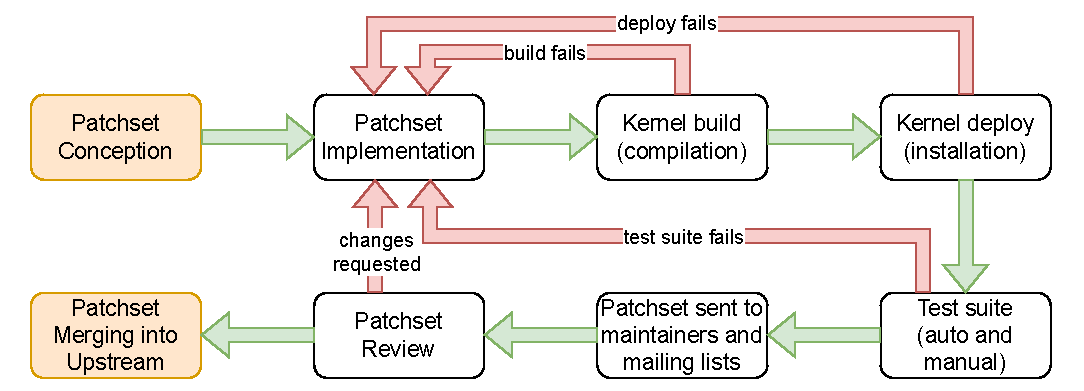
\includegraphics[width=1\linewidth, 
    clip=true, trim= 0px 0px 0px 0px]
    {figs/patchset-development-workflow.pdf}}
    \caption{Concept map of the patchset development workflow.}
    \label{fig:patchset-dev-workflow}
\end{figure}

\begin{figure}[ht]
    \centering
    \fbox{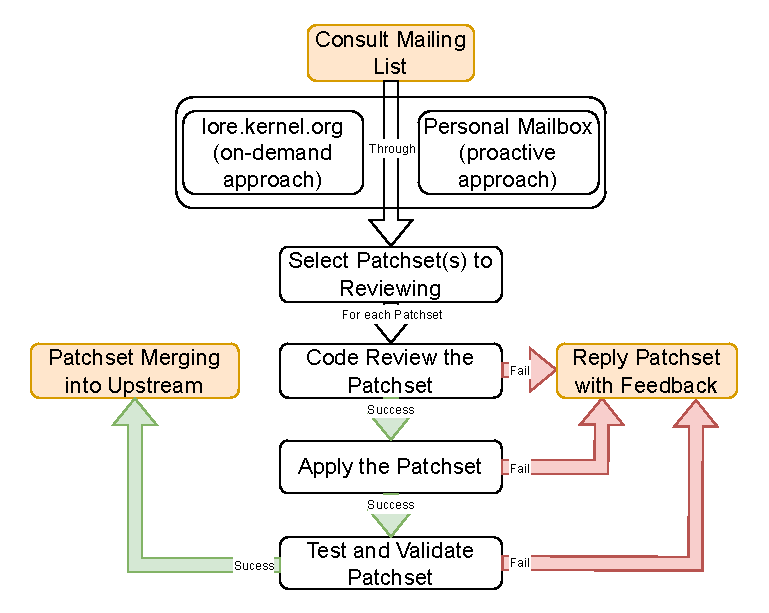
\includegraphics[width=1\linewidth, 
    clip=true, trim= 0px 0px 0px 0px]
    {figs/patchset-reviewing-workflow.pdf}}
    \caption{Concept map of the patchset reviewing workflow.}
    \label{fig:patchset-dev-workflow}
\end{figure}
